% Options for packages loaded elsewhere
\PassOptionsToPackage{unicode}{hyperref}
\PassOptionsToPackage{hyphens}{url}
%
\documentclass[
]{article}
\usepackage{amsmath,amssymb}
\usepackage{lmodern}
\usepackage{iftex}
\ifPDFTeX
  \usepackage[T1]{fontenc}
  \usepackage[utf8]{inputenc}
  \usepackage{textcomp} % provide euro and other symbols
\else % if luatex or xetex
  \usepackage{unicode-math}
  \defaultfontfeatures{Scale=MatchLowercase}
  \defaultfontfeatures[\rmfamily]{Ligatures=TeX,Scale=1}
\fi
% Use upquote if available, for straight quotes in verbatim environments
\IfFileExists{upquote.sty}{\usepackage{upquote}}{}
\IfFileExists{microtype.sty}{% use microtype if available
  \usepackage[]{microtype}
  \UseMicrotypeSet[protrusion]{basicmath} % disable protrusion for tt fonts
}{}
\makeatletter
\@ifundefined{KOMAClassName}{% if non-KOMA class
  \IfFileExists{parskip.sty}{%
    \usepackage{parskip}
  }{% else
    \setlength{\parindent}{0pt}
    \setlength{\parskip}{6pt plus 2pt minus 1pt}}
}{% if KOMA class
  \KOMAoptions{parskip=half}}
\makeatother
\usepackage{xcolor}
\IfFileExists{xurl.sty}{\usepackage{xurl}}{} % add URL line breaks if available
\IfFileExists{bookmark.sty}{\usepackage{bookmark}}{\usepackage{hyperref}}
\hypersetup{
  pdftitle={First Implementation of QuickPay (2009-2012)},
  hidelinks,
  pdfcreator={LaTeX via pandoc}}
\urlstyle{same} % disable monospaced font for URLs
\usepackage[margin=1in]{geometry}
\usepackage{graphicx}
\makeatletter
\def\maxwidth{\ifdim\Gin@nat@width>\linewidth\linewidth\else\Gin@nat@width\fi}
\def\maxheight{\ifdim\Gin@nat@height>\textheight\textheight\else\Gin@nat@height\fi}
\makeatother
% Scale images if necessary, so that they will not overflow the page
% margins by default, and it is still possible to overwrite the defaults
% using explicit options in \includegraphics[width, height, ...]{}
\setkeys{Gin}{width=\maxwidth,height=\maxheight,keepaspectratio}
% Set default figure placement to htbp
\makeatletter
\def\fps@figure{htbp}
\makeatother
\setlength{\emergencystretch}{3em} % prevent overfull lines
\providecommand{\tightlist}{%
  \setlength{\itemsep}{0pt}\setlength{\parskip}{0pt}}
\setcounter{secnumdepth}{5}
\usepackage{booktabs,longtable,dcolumn} \usepackage{multirow,array} \usepackage{wrapfig,float} \floatplacement{figure}{H}
\ifLuaTeX
  \usepackage{selnolig}  % disable illegal ligatures
\fi

\title{First Implementation of QuickPay (2009-2012)}
\author{}
\date{\vspace{-2.5em}Nov 09, 2021}

\begin{document}
\maketitle

\hypertarget{delays-over-time}{%
\section{Delays over Time}\label{delays-over-time}}

\begin{itemize}
\tightlist
\item
  Sample restricted to projects for which start dates matches the one in
  API

  \begin{itemize}
  \tightlist
  \item
    This is done by using first reported ``action\_date'' and
    ``date\_signed''
  \end{itemize}
\item
  \(DelayRate_{it}=Deadline_{i,t} - Deadline_{i,t-1}\)
\end{itemize}

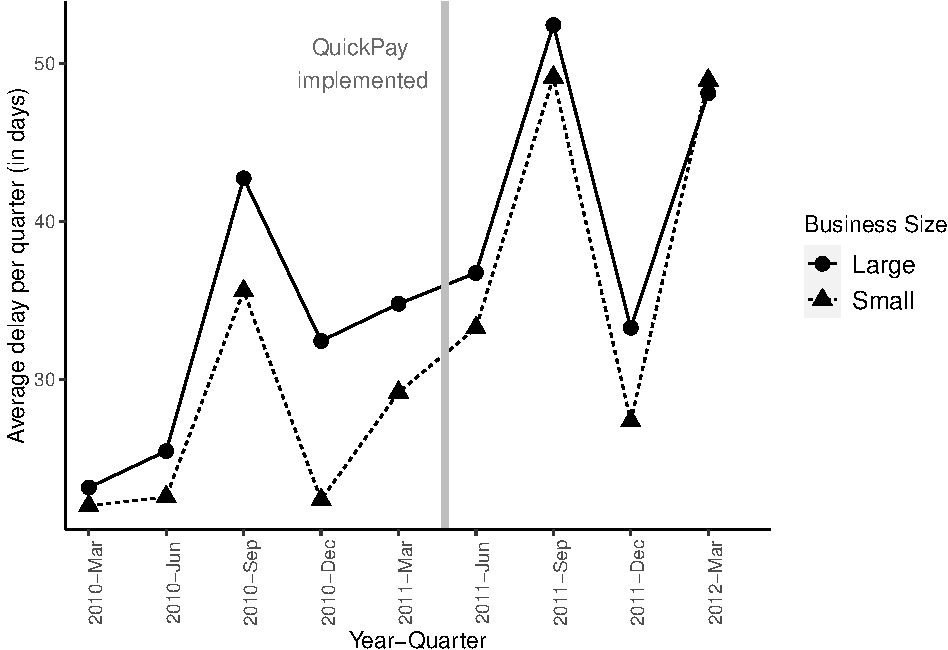
\includegraphics{qp_first_implementation_files/figure-latex/plot-1.pdf}

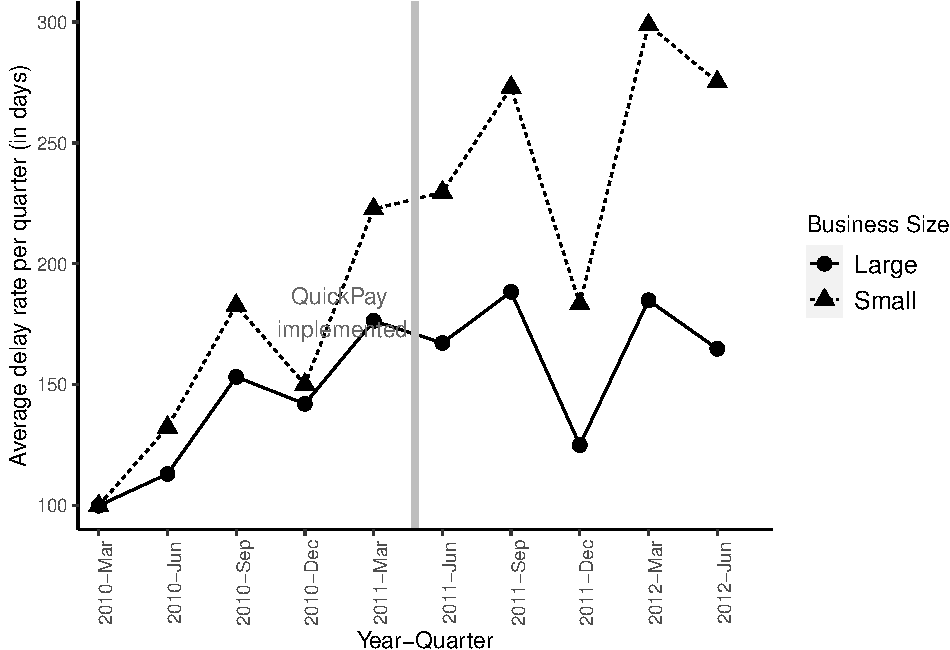
\includegraphics{qp_first_implementation_files/figure-latex/normalized_plot-1.pdf}
\# Notation

\begin{itemize}
\tightlist
\item
  Project \(i\), Year-Quarter \(t\)
\item
  \(X_i\) denotes project level controls: initial duration, initial
  budget, number of offers received
\item
  \(\mu_t,\theta_{firm},\lambda_{task}\): Year-Quarter, Firm, and
  Product/Service code Fixed effects
\item
  All continuous variables are winsorized at the 5\% level
  \[ Treat_i = \begin{cases} 1, \text{ if project } i \text{ is a small business}\\
  0, \text{ otherwise} \end{cases}\]
  \[ Post_t = \begin{cases} 1, \text{ if year-quarter } t > \text{ April 27, 2011}\\
  0, \text{ otherwise} \end{cases}\]
\end{itemize}

\hypertarget{summary-statistics}{%
\section{Summary Statistics}\label{summary-statistics}}

\hypertarget{parallel-trends-test}{%
\section{Parallel Trends Test}\label{parallel-trends-test}}

Let \(Time\) denote \(q\)-th quarter since the beginning of time
horizon. For \(Post_t =0\), we run the following regression:
\[ Delay_{it} = \alpha+\beta_0 Treat_i + \beta_1 (Treat_i \times Time) + \beta_2 X_i + \mu_t + \theta_{firm} + \lambda_{task} +\epsilon_{it}\]
The coefficient of interest is \(\beta_1\). If this is significant, we
would find evidence of a linear time trend before quickpay
implementation -- violating the parallel trends assumption.

\begin{table}[H] \centering 
  \caption{Linear Time Trend Before QuickPay} 
  \label{} 
\small 
\begin{tabular}{@{\extracolsep{5pt}}lc} 
\\[-1.8ex]\hline 
\hline \\[-1.8ex] 
 & \multicolumn{1}{c}{\textit{Dependent variable:}} \\ 
\cline{2-2} 
\\[-1.8ex] & $Delay_{it}$ (in days) \\ 
\hline \\[-1.8ex] 
 $Treat_i$ & $-$1.71$^{**}$ \\ 
  & (0.72) \\ 
  & \\ 
 $Treat_i \times Time$ & 0.01 \\ 
  & (0.13) \\ 
  & \\ 
\hline \\[-1.8ex] 
Fixed effects & Firm, Task, and Year-Quarter \\ 
Controls & Budget, Duration, Bids, Project Age \\ 
Observations & 99,007 \\ 
R$^{2}$ & 0.25 \\ 
Adjusted R$^{2}$ & 0.16 \\ 
\hline 
\hline \\[-1.8ex] 
\textit{Note:}  & \multicolumn{1}{r}{$^{*}$p$<$0.1; $^{**}$p$<$0.05; $^{***}$p$<$0.01} \\ 
 & \multicolumn{1}{r}{Each observation is a project-quarter.} \\ 
 & \multicolumn{1}{r}{SEs are robust and clustered at the project level.} \\ 
 & \multicolumn{1}{r}{Observations are for quarters before quickpay.} \\ 
\end{tabular} 
\end{table}

\hypertarget{baseline-regressions}{%
\section{Baseline Regressions}\label{baseline-regressions}}

\[ Delay_{it} = \alpha+\beta_0 Treat_i + \beta_1 Post_t + \beta_2 (Treat_i \times Post_t) + \epsilon_{it}\]

\[ \begin{aligned} Delay_{it} &=& \alpha+\beta_0 Treat_i + \beta_1 Post_t + \beta_2 (Treat_i \times Post_t)\\
&+&  X_i + (Post_t \times X_i) + \mu_t + \theta_{firm} + \lambda_{task}+ \epsilon_{it}
\end{aligned}\]

\begin{table}[H] \centering 
  \caption{Quickpay 2009-2011} 
  \label{} 
\small 
\begin{tabular}{@{\extracolsep{-2pt}}lccccc} 
\\[-1.8ex]\hline 
\hline \\[-1.8ex] 
\\[-1.8ex] & \multicolumn{5}{c}{$Delay_{it}$ (in days)} \\ 
\\[-1.8ex] & (1) & (2) & (3) & (4) & (5)\\ 
\hline \\[-1.8ex] 
 $Treat_i$ & $-$3.34$^{***}$ & $-$2.26$^{***}$ & $-$2.28$^{***}$ & $-$1.94$^{***}$ & $-$1.87$^{***}$ \\ 
  & (0.15) & (0.15) & (0.15) & (0.15) & (0.34) \\ 
  & & & & & \\ 
 $Post_t$ & 1.02$^{***}$ & $-$1.86$^{***}$ &  &  &  \\ 
  & (0.15) & (0.31) &  &  &  \\ 
  & & & & & \\ 
 $Treat_i \times Post_t$ & 1.34$^{***}$ & 1.57$^{***}$ & 1.59$^{***}$ & 1.39$^{***}$ & 1.48$^{***}$ \\ 
  & (0.19) & (0.19) & (0.19) & (0.19) & (0.20) \\ 
  & & & & & \\ 
 Constant & 8.35$^{***}$ & 14.51$^{***}$ &  &  &  \\ 
  & (0.12) & (0.23) &  &  &  \\ 
  & & & & & \\ 
\hline \\[-1.8ex] 
Duration, Budget, Bids & No & Yes & Yes & Yes & Yes \\ 
$Post_t \times$  (Duration, Budget, Bids) & No & Yes & Yes & Yes & Yes \\ 
Project Age Tercile & No & Yes & Yes & Yes & Yes \\ 
Year-Quarter Fixed Effects & No & No & Yes & Yes & Yes \\ 
Task Fixed Effects & No & No & No & Yes & Yes \\ 
Firm Fixed Effects & No & No & No & No & Yes \\ 
Observations & 287,530 & 263,488 & 263,488 & 263,488 & 263,488 \\ 
R$^{2}$ & 0.004 & 0.08 & 0.08 & 0.11 & 0.18 \\ 
Adjusted R$^{2}$ & 0.004 & 0.08 & 0.08 & 0.10 & 0.13 \\ 
\hline 
\hline \\[-1.8ex] 
\textit{Note:}  & \multicolumn{5}{r}{$^{*}$p$<$0.1; $^{**}$p$<$0.05; $^{***}$p$<$0.01} \\ 
 & \multicolumn{5}{r}{Each observation is a project-quarter.} \\ 
 & \multicolumn{5}{r}{SEs are robust and clustered at the project level.} \\ 
\end{tabular} 
\end{table}

\hypertarget{competition}{%
\section{Competition}\label{competition}}

\[ Competition_i = \begin{cases} 1, \text{ if project was subject to full and open competition}\\ 
                       \text{(extent competed code is not B, C, G, E, or "")}\\
0, \text{ otherwise} \end{cases}\]

\textbf{Hypothesis:}

\begin{itemize}
\tightlist
\item
  QuickPay increased competition for small projects.
\item
  This led to more aggressive bids. That is, contractors quoted
  unrealistically small timelines for the projects.
\item
  As a result, we should see ``artificial delays'' on these projects as
  they revert to their realistic timelines later.
\item
  \textbf{Note:} This hypothesis only applies to projects that were
  signed after QuickPay. We, therefore, need the effect coming from
  projects that were signed after QuickPay.
\end{itemize}

\hypertarget{impact-on-bids-duration-and-budget}{%
\subsection{Impact on bids, duration, and
budget}\label{impact-on-bids-duration-and-budget}}

\[ \begin{aligned}
y_{it} &=& \beta_0 + \beta_1 Treat_i + \beta_2 (Treat_i \times Post_t) +\mu_t+ \lambda_{task}+ e_{it}
\end{aligned}\]

where \(y_{it}\) denotes bids, duration, or budget of project \(i\)
signed in quarter \(t\).

\begin{itemize}
\tightlist
\item
  \(Post_t\) is a dummy that equals one if \(t\) is a quarter after
  QuickPay was launched.
\item
  \(\mu_t\) denotes fixed effects for the quarter in which the project
  was signed.
\end{itemize}

\begin{table}[H] \centering 
  \caption{Effect of Competition After QuickPay: Quickpay 2009-2011} 
  \label{} 
\small 
\begin{tabular}{@{\extracolsep{0pt}}lccc} 
\\[-1.8ex]\hline 
\hline \\[-1.8ex] 
\\[-1.8ex] & $NumberOfBids_{it}$ & $InitialDuration_{it}$ & $InitialBudget_{it}$ \\ 
\\[-1.8ex] & (1) & (2) & (3)\\ 
\hline \\[-1.8ex] 
 $Treat_i$ & 0.89$^{***}$ & $-$7.33$^{***}$ & $-$10,203.21$^{***}$ \\ 
  & (0.09) & (0.70) & (1,103.25) \\ 
  & & & \\ 
 $Treat_i \times Post_t$ & 0.27$^{**}$ & $-$3.26$^{***}$ & $-$22,048.85$^{***}$ \\ 
  & (0.12) & (0.98) & (1,580.03) \\ 
  & & & \\ 
\hline \\[-1.8ex] 
Task fixed effects & Yes & Yes & Yes \\ 
Time fixed effects & Yes & Yes & Yes \\ 
Observations & 227,318 & 220,524 & 227,358 \\ 
R$^{2}$ & 0.25 & 0.20 & 0.27 \\ 
Adjusted R$^{2}$ & 0.24 & 0.19 & 0.26 \\ 
\hline 
\hline \\[-1.8ex] 
\textit{Note:}  & \multicolumn{3}{r}{$^{*}$p$<$0.1; $^{**}$p$<$0.05; $^{***}$p$<$0.01} \\ 
 & \multicolumn{3}{r}{Each observation is a project-quarter.} \\ 
 & \multicolumn{3}{r}{SEs are robust and clustered at the project level.} \\ 
 & \multicolumn{3}{r}{Sample restricted to fully competed projects.} \\ 
\end{tabular} 
\end{table}

\hypertarget{impact-on-bids}{%
\subsection{Impact on bids}\label{impact-on-bids}}

\begin{table}[H] \centering 
  \caption{Effect of Competition After QuickPay: Quickpay 2009-2011} 
  \label{} 
\small 
\begin{tabular}{@{\extracolsep{-2pt}}lccc} 
\\[-1.8ex]\hline 
\hline \\[-1.8ex] 
\\[-1.8ex] & \multicolumn{3}{c}{$NumberOfBids_{it}$} \\ 
\\[-1.8ex] & (1) & (2) & (3)\\ 
\hline \\[-1.8ex] 
 $Treat_i$ & 0.25$^{***}$ & 0.25$^{***}$ & 0.89$^{***}$ \\ 
  & (0.10) & (0.10) & (0.09) \\ 
  & & & \\ 
 $Post_t$ & $-$0.34$^{***}$ &  &  \\ 
  & (0.11) &  &  \\ 
  & & & \\ 
 $Treat_i \times Post_t$ & 0.30$^{**}$ & 0.30$^{**}$ & 0.27$^{**}$ \\ 
  & (0.13) & (0.13) & (0.12) \\ 
  & & & \\ 
 Constant & 5.07$^{***}$ &  &  \\ 
  & (0.08) &  &  \\ 
  & & & \\ 
\hline \\[-1.8ex] 
Year-Quarter Fixed Effects & No & Yes & Yes \\ 
Task Fixed Effects & No & No & Yes \\ 
Observations & 227,318 & 227,318 & 227,318 \\ 
R$^{2}$ & 0.0002 & 0.0003 & 0.25 \\ 
Adjusted R$^{2}$ & 0.0002 & 0.0003 & 0.24 \\ 
\hline 
\hline \\[-1.8ex] 
\textit{Note:}  & \multicolumn{3}{r}{$^{*}$p$<$0.1; $^{**}$p$<$0.05; $^{***}$p$<$0.01} \\ 
 & \multicolumn{3}{r}{Each observation is a project-quarter.} \\ 
 & \multicolumn{3}{r}{SEs are robust and clustered at the project level.} \\ 
 & \multicolumn{3}{r}{Sample restricted to fully competed projects.} \\ 
\end{tabular} 
\end{table}

\hypertarget{impact-on-initial-duration}{%
\subsection{Impact on Initial
Duration}\label{impact-on-initial-duration}}

\begin{table}[H] \centering 
  \caption{Effect of Competition After QuickPay: Quickpay 2009-2011} 
  \label{} 
\small 
\begin{tabular}{@{\extracolsep{-2pt}}lcccc} 
\\[-1.8ex]\hline 
\hline \\[-1.8ex] 
\\[-1.8ex] & \multicolumn{4}{c}{$InitialDuration_{it}$} \\ 
\\[-1.8ex] & (1) & (2) & (3) & (4)\\ 
\hline \\[-1.8ex] 
 $Treat_i$ & $-$18.02$^{***}$ & $-$17.61$^{***}$ & $-$7.33$^{***}$ & $-$6.65$^{***}$ \\ 
  & (0.70) & (0.70) & (0.70) & (1.62) \\ 
  & & & & \\ 
 $Post_t$ & 1.27 &  &  &  \\ 
  & (0.88) &  &  &  \\ 
  & & & & \\ 
 $Treat_i \times Post_t$ & 2.84$^{***}$ & 2.52$^{**}$ & $-$3.26$^{***}$ & $-$2.04$^{**}$ \\ 
  & (1.06) & (1.06) & (0.98) & (0.95) \\ 
  & & & & \\ 
 Constant & 136.56$^{***}$ &  &  &  \\ 
  & (0.58) &  &  &  \\ 
  & & & & \\ 
\hline \\[-1.8ex] 
Year-Quarter Fixed Effects & No & Yes & Yes & Yes \\ 
Task Fixed Effects & No & No & Yes & Yes \\ 
Firm Fixed Effects & No & No & No & Yes \\ 
Observations & 220,524 & 220,524 & 220,524 & 220,523 \\ 
R$^{2}$ & 0.01 & 0.01 & 0.20 & 0.50 \\ 
Adjusted R$^{2}$ & 0.01 & 0.01 & 0.19 & 0.45 \\ 
\hline 
\hline \\[-1.8ex] 
\textit{Note:}  & \multicolumn{4}{r}{$^{*}$p$<$0.1; $^{**}$p$<$0.05; $^{***}$p$<$0.01} \\ 
 & \multicolumn{4}{r}{Each observation is a project-quarter.} \\ 
 & \multicolumn{4}{r}{SEs are robust and clustered at the project level.} \\ 
 & \multicolumn{4}{r}{Sample restricted to fully competed projects.} \\ 
\end{tabular} 
\end{table}

\hypertarget{impact-on-initial-budget}{%
\subsection{Impact on Initial Budget}\label{impact-on-initial-budget}}

\begin{table}[H] \centering 
  \caption{Effect of Competition After QuickPay: Quickpay 2009-2011} 
  \label{} 
\small 
\begin{tabular}{@{\extracolsep{-2pt}}lcccc} 
\\[-1.8ex]\hline 
\hline \\[-1.8ex] 
\\[-1.8ex] & \multicolumn{4}{c}{$InitialBudget_{it}$} \\ 
\\[-1.8ex] & (1) & (2) & (3) & (4)\\ 
\hline \\[-1.8ex] 
 $Treat_i$ & $-$64,224.13$^{***}$ & $-$60,124.82$^{***}$ & $-$10,203.21$^{***}$ & $-$1,845.16 \\ 
  & (1,020.96) & (1,135.76) & (1,103.25) & (2,564.91) \\ 
  & & & & \\ 
 $Post_t$ & 23.31$^{***}$ &  &  &  \\ 
  & (2.08) &  &  &  \\ 
  & & & & \\ 
 $Treat_i \times Post_t$ & $-$7,454.09$^{***}$ & $-$17,016.07$^{***}$ & $-$22,048.85$^{***}$ & $-$19,847.89$^{***}$ \\ 
  & (1,339.70) & (1,810.34) & (1,580.03) & (1,548.88) \\ 
  & & & & \\ 
 Constant & $-$217,694.10$^{***}$ &  &  &  \\ 
  & (31,218.93) &  &  &  \\ 
  & & & & \\ 
\hline \\[-1.8ex] 
Year-Quarter Fixed Effects & No & Yes & Yes & Yes \\ 
Task Fixed Effects & No & No & Yes & Yes \\ 
Firm Fixed Effects & No & No & No & Yes \\ 
Observations & 227,358 & 227,358 & 227,358 & 227,357 \\ 
R$^{2}$ & 0.03 & 0.04 & 0.27 & 0.50 \\ 
Adjusted R$^{2}$ & 0.03 & 0.04 & 0.26 & 0.45 \\ 
\hline 
\hline \\[-1.8ex] 
\textit{Note:}  & \multicolumn{4}{r}{$^{*}$p$<$0.1; $^{**}$p$<$0.05; $^{***}$p$<$0.01} \\ 
 & \multicolumn{4}{r}{Each observation is a project-quarter.} \\ 
 & \multicolumn{4}{r}{SEs are robust and clustered at the project level.} \\ 
 & \multicolumn{4}{r}{Sample restricted to fully competed projects.} \\ 
\end{tabular} 
\end{table}

\hypertarget{impact-on-delays}{%
\subsection{Impact on delays}\label{impact-on-delays}}

Define
\[ SA_i = \begin{cases} 1, \text{ if project was signed after QuickPay}\\
0, \text{ otherwise} \end{cases}\]

\[ SB_i = \begin{cases} 1, \text{ if project was signed before QuickPay}\\
0, \text{ otherwise} \end{cases}\]

\hypertarget{subsample-model}{%
\subsubsection{Subsample model}\label{subsample-model}}

For a subsample of competitive or noncompetitive projects:

\[ \begin{aligned} Delay_{it} &=& \beta_0 +\beta_1 Treat_i+ \beta_2 SA_i+ \beta_3 Post_t \\&+& \beta_4 (Treat_i \times Post_t \times SA_i )+\beta_5 (Treat_i \times Post_t \times SB_i )+\epsilon_{it} \end{aligned} \]

\begin{itemize}
\tightlist
\item
  According to our hypothesis, \(\beta_4\) should be positive and
  significant for competitive projects, and insignificant for
  non-competitive projects.
\item
  In the following regressions, we also control for the project's age.
  Project's age is defined as the number of quarters since it first
  showed up in the sample. We include the terciles of project's age as a
  control variable.
\end{itemize}

\begin{table}[H] \centering 
  \caption{Subsample of Competitive Projects: Quickpay 2009-2011} 
  \label{} 
\small 
\begin{tabular}{@{\extracolsep{-2pt}}lccccc} 
\\[-1.8ex]\hline 
\hline \\[-1.8ex] 
\\[-1.8ex] & \multicolumn{5}{c}{$Delay_{it}$ (in days)} \\ 
\\[-1.8ex] & (1) & (2) & (3) & (4) & (5)\\ 
\hline \\[-1.8ex] 
 $Treat_i$ & $-$4.23$^{***}$ & $-$2.75$^{***}$ & $-$2.82$^{***}$ & $-$1.98$^{***}$ & $-$2.08$^{***}$ \\ 
  & (0.17) & (0.16) & (0.16) & (0.17) & (0.39) \\ 
  & & & & & \\ 
 $SA_i$ & $-$5.24$^{***}$ & $-$3.39$^{***}$ & $-$5.60$^{***}$ & $-$5.54$^{***}$ & $-$4.89$^{***}$ \\ 
  & (0.24) & (0.24) & (0.27) & (0.27) & (0.28) \\ 
  & & & & & \\ 
 $Post_t$ & 4.18$^{***}$ & 0.39 &  &  &  \\ 
  & (0.22) & (0.38) &  &  &  \\ 
  & & & & & \\ 
 $Treat_i \times SB_i \times Post_t$ & $-$0.21 & 0.97$^{***}$ & 1.12$^{***}$ & 1.11$^{***}$ & 1.21$^{***}$ \\ 
  & (0.27) & (0.29) & (0.29) & (0.28) & (0.29) \\ 
  & & & & & \\ 
 $Treat_i \times SA_i \times Post_t$ & 2.03$^{***}$ & 1.91$^{***}$ & 1.89$^{***}$ & 1.98$^{***}$ & 1.95$^{***}$ \\ 
  & (0.25) & (0.24) & (0.24) & (0.23) & (0.24) \\ 
  & & & & & \\ 
 Constant & 8.84$^{***}$ & 15.05$^{***}$ &  &  &  \\ 
  & (0.14) & (0.26) &  &  &  \\ 
  & & & & & \\ 
\hline \\[-1.8ex] 
Duration, Budget, Bids & No & Yes & Yes & Yes & Yes \\ 
$Post_t \times $  (Duration, Budget, Bids) & No & Yes & Yes & Yes & Yes \\ 
Project age & No & Yes & Yes & Yes & Yes \\ 
Year-Quarter Fixed Effects & No & No & Yes & Yes & Yes \\ 
Task Fixed Effects & No & No & No & Yes & Yes \\ 
Firm Fixed Effects & No & No & No & No & Yes \\ 
Observations & 234,573 & 214,421 & 214,421 & 214,421 & 214,421 \\ 
R$^{2}$ & 0.01 & 0.08 & 0.09 & 0.12 & 0.19 \\ 
Adjusted R$^{2}$ & 0.01 & 0.08 & 0.09 & 0.11 & 0.14 \\ 
\hline 
\hline \\[-1.8ex] 
\textit{Note:}  & \multicolumn{5}{r}{$^{*}$p$<$0.1; $^{**}$p$<$0.05; $^{***}$p$<$0.01} \\ 
 & \multicolumn{5}{r}{Each observation is a project-quarter.} \\ 
 & \multicolumn{5}{r}{SEs are robust and clustered at the project level.} \\ 
 & \multicolumn{5}{r}{Sample restricted to fully competed projects.} \\ 
\end{tabular} 
\end{table}

\begin{table}[H] \centering 
  \caption{Subsample of Non-competitive Projects: Quickpay 2009-2011} 
  \label{} 
\small 
\begin{tabular}{@{\extracolsep{-2pt}}lcccc} 
\\[-1.8ex]\hline 
\hline \\[-1.8ex] 
\\[-1.8ex] & \multicolumn{4}{c}{$Delay_{it}$ (in days)} \\ 
\\[-1.8ex] & (1) & (2) & (3) & (4)\\ 
\hline \\[-1.8ex] 
 $Treat_i$ & 1.30$^{***}$ & 0.60 & 0.65$^{*}$ & $-$1.43$^{***}$ \\ 
  & (0.37) & (0.37) & (0.37) & (0.40) \\ 
  & & & & \\ 
 $SA_i$ & $-$1.80$^{***}$ & $-$0.52 & $-$1.69$^{***}$ & $-$1.79$^{***}$ \\ 
  & (0.32) & (0.32) & (0.41) & (0.41) \\ 
  & & & & \\ 
 $Post_t$ & 0.64$^{**}$ & $-$0.04 &  &  \\ 
  & (0.32) & (0.81) &  &  \\ 
  & & & & \\ 
 $Treat_i \times SB_i \times Post_t$ & 2.78$^{***}$ & 3.16$^{***}$ & 3.17$^{***}$ & 3.29$^{***}$ \\ 
  & (0.56) & (0.60) & (0.60) & (0.61) \\ 
  & & & & \\ 
 $Treat_i \times SA_i \times Post_t$ & 0.71 & $-$0.11 & $-$0.02 & 0.12 \\ 
  & (0.52) & (0.51) & (0.51) & (0.52) \\ 
  & & & & \\ 
 Constant & 6.29$^{***}$ & 13.61$^{***}$ &  &  \\ 
  & (0.25) & (0.63) &  &  \\ 
  & & & & \\ 
\hline \\[-1.8ex] 
Duration, Budget, Bids & No & Yes & Yes & Yes \\ 
$Post_t \times $  (Duration, Budget, Bids) & No & Yes & Yes & Yes \\ 
Project age & No & Yes & Yes & Yes \\ 
Year-Quarter Fixed Effects & No & No & Yes & Yes \\ 
Task Fixed Effects & No & No & No & Yes \\ 
Observations & 52,957 & 49,067 & 49,067 & 49,067 \\ 
R$^{2}$ & 0.01 & 0.07 & 0.07 & 0.11 \\ 
Adjusted R$^{2}$ & 0.005 & 0.07 & 0.07 & 0.09 \\ 
\hline 
\hline \\[-1.8ex] 
\textit{Note:}  & \multicolumn{4}{r}{$^{*}$p$<$0.1; $^{**}$p$<$0.05; $^{***}$p$<$0.01} \\ 
 & \multicolumn{4}{r}{Each observation is a project-quarter.} \\ 
 & \multicolumn{4}{r}{SEs are robust and clustered at the project level.} \\ 
 & \multicolumn{4}{r}{Sample restricted to non-competed projects.} \\ 
\end{tabular} 
\end{table}

\hypertarget{four-way-interaction}{%
\subsubsection{Four-way interaction}\label{four-way-interaction}}

We run the following model:

\[\begin{aligned} Delay_{it} &=& \beta_0 +\beta_1 Treat_i+ \beta_2 StartedAfterQP_i+ \beta_3 Post_t+ \beta_4 Competitive_i\\ && +  \beta_5 (Treat_i \times Competitive_i) + \beta_6 (Post_t \times Competitive_i)\\ && +  \beta_7 (StartedAfterQP_i \times Competitive_i) +\beta_8 (Treat_i \times Post_t)\\ && + \beta_9 (Treat_i \times Post_t \times Competitive_i) \\ && + \beta_{10} (Treat_i \times Post_t \times StartedAfterQP_i )\\ && + \beta_{11} (Treat_i \times Post_t \times StartedAfterQP_i \times Competitive_i) + \epsilon_{it} \end{aligned}\]

\textbf{Interpretation:}

\begin{itemize}
\tightlist
\item
  \(\beta_9\) is the difference between treatment effect for competitive
  and non-competitive projects signed before quickpay.
\item
  \(\beta_9 + \beta_{11}\) is the difference between treatment effect
  for competitive and non-competitive projects signed \emph{after}
  quickpay.
\item
  \(\beta_{11}\) is our coefficient of interest because it tells us how
  much of the difference is there due to ``aggressive bidding'' after
  the policy.
\end{itemize}

\begin{table}[H] \centering 
  \caption{Effect of Competition After QuickPay: Quickpay 2009-2011} 
  \label{} 
\small 
\begin{tabular}{@{\extracolsep{-3pt}}lcccccc} 
\\[-1.8ex]\hline 
\hline \\[-1.8ex] 
\\[-1.8ex] & \multicolumn{6}{c}{$Delay_{it}$ (in days)} \\ 
\\[-1.8ex] & (1) & (2) & (3) & (4) & (5) & (6)\\ 
\hline \\[-1.8ex] 
 $Treat_i$ & 1.30$^{***}$ & 0.53 & 0.41 & 0.47 & $-$1.51$^{***}$ & $-$2.34$^{***}$ \\ 
  & (0.37) & (0.37) & (0.37) & (0.37) & (0.38) & (0.53) \\ 
  & & & & & & \\ 
 $StartedAfterQP_i$ & $-$1.80$^{***}$ & $-$2.80$^{***}$ & 0.08 & $-$1.97$^{***}$ & $-$2.28$^{***}$ & $-$2.33$^{***}$ \\ 
  & (0.32) & (0.32) & (0.31) & (0.33) & (0.34) & (0.33) \\ 
  & & & & & & \\ 
 $Competitive_i$ & 2.56$^{***}$ & 1.08$^{***}$ & 1.04$^{***}$ & 1.13$^{***}$ & $-$0.04 & $-$0.88$^{**}$ \\ 
  & (0.28) & (0.28) & (0.28) & (0.28) & (0.29) & (0.35) \\ 
  & & & & & & \\ 
 $Post_t$ & 0.64$^{**}$ & 0.64 & $-$2.10$^{***}$ &  &  &  \\ 
  & (0.32) & (0.43) & (0.43) &  &  &  \\ 
  & & & & & & \\ 
 $Treat_i \times Competitive_i$ & $-$5.52$^{***}$ & $-$3.83$^{***}$ & $-$3.21$^{***}$ & $-$3.33$^{***}$ & $-$0.58 & 0.53 \\ 
  & (0.41) & (0.41) & (0.40) & (0.40) & (0.41) & (0.50) \\ 
  & & & & & & \\ 
 $Post_t \times Competitive_i$ & 3.54$^{***}$ & 2.90$^{***}$ & 2.86$^{***}$ & 2.89$^{***}$ & 1.88$^{***}$ & 1.88$^{***}$ \\ 
  & (0.39) & (0.40) & (0.40) & (0.40) & (0.40) & (0.42) \\ 
  & & & & & & \\ 
 $StartedAfterQP_i \times Competitive_i$ & $-$3.44$^{***}$ & $-$3.65$^{***}$ & $-$3.62$^{***}$ & $-$3.56$^{***}$ & $-$3.16$^{***}$ & $-$2.35$^{***}$ \\ 
  & (0.40) & (0.39) & (0.39) & (0.39) & (0.39) & (0.39) \\ 
  & & & & & & \\ 
 $Treat_i \times Post_t$ & 2.78$^{***}$ & 3.15$^{***}$ & 3.12$^{***}$ & 3.20$^{***}$ & 2.81$^{***}$ & 3.41$^{***}$ \\ 
  & (0.56) & (0.60) & (0.60) & (0.60) & (0.60) & (0.63) \\ 
  & & & & & & \\ 
 $Treat_i \times Post_t \times Competitive_i$ & $-$2.98$^{***}$ & $-$1.99$^{***}$ & $-$2.15$^{***}$ & $-$2.09$^{***}$ & $-$1.71$^{***}$ & $-$2.28$^{***}$ \\ 
  & (0.62) & (0.67) & (0.66) & (0.66) & (0.66) & (0.69) \\ 
  & & & & & & \\ 
 $Treat_i \times Post_t \times StartedAfterQP_i$ & $-$2.07$^{***}$ & $-$3.28$^{***}$ & $-$3.31$^{***}$ & $-$3.24$^{***}$ & $-$3.07$^{***}$ & $-$2.75$^{***}$ \\ 
  & (0.59) & (0.61) & (0.60) & (0.60) & (0.60) & (0.61) \\ 
  & & & & & & \\ 
 $Treat_i \times Post_t \times StartedAfterQP_i \times Competitive_i$ & 4.31$^{***}$ & 4.17$^{***}$ & 4.26$^{***}$ & 4.03$^{***}$ & 3.97$^{***}$ & 3.44$^{***}$ \\ 
  & (0.66) & (0.68) & (0.67) & (0.67) & (0.67) & (0.68) \\ 
  & & & & & & \\ 
 Constant & 6.29$^{***}$ & 16.06$^{***}$ & 13.85$^{***}$ &  &  &  \\ 
  & (0.25) & (0.32) & (0.31) &  &  &  \\ 
  & & & & & & \\ 
\hline \\[-1.8ex] 
Duration, Budget, Bids & No & Yes & Yes & Yes & Yes & Yes \\ 
$Post_t \times $  (Duration, Budget, Bids) & No & Yes & Yes & Yes & Yes & Yes \\ 
Project age & No & No & Yes & Yes & Yes & Yes \\ 
Year-Quarter Fixed Effects & No & No & No & Yes & Yes & Yes \\ 
Task Fixed Effects & No & No & No & No & Yes & Yes \\ 
Firm Fixed Effects & No & No & No & No & No & Yes \\ 
Observations & 287,530 & 263,488 & 263,488 & 263,488 & 263,488 & 263,488 \\ 
R$^{2}$ & 0.01 & 0.06 & 0.08 & 0.08 & 0.11 & 0.18 \\ 
Adjusted R$^{2}$ & 0.01 & 0.06 & 0.08 & 0.08 & 0.11 & 0.13 \\ 
\hline 
\hline \\[-1.8ex] 
\textit{Note:}  & \multicolumn{6}{r}{$^{*}$p$<$0.1; $^{**}$p$<$0.05; $^{***}$p$<$0.01} \\ 
 & \multicolumn{6}{r}{Each observation is a project-quarter.} \\ 
 & \multicolumn{6}{r}{SEs are robust and clustered at the project level.} \\ 
\end{tabular} 
\end{table}

\hypertarget{impact-of-firms-financial-constraints}{%
\section{Impact of Firm's Financial
Constraints}\label{impact-of-firms-financial-constraints}}

\hypertarget{contract-financing}{%
\subsection{Contract Financing}\label{contract-financing}}

\[ CF_i = \begin{cases} 1, \text{ if project } i \text{ receives contract financing}\\
0, \text{ otherwise} \end{cases}\]

\[ \begin{aligned}
Delay_{it} &=& \alpha+\beta_0 Treat_i + \beta_1 Post_t + \beta_2 (Treat_i \times Post_t) \\
&+&\beta_3 CF_i + \beta_4 (CF_i \times Post_t) + \beta_5 (Treat_i \times Post_t \times CF_i) \\ 
&+&X_i + (Post_t \times X_i) + \mu_t + \theta_{firm} + \lambda_{task}+ \epsilon_{it}
\end{aligned}\]

\begin{table}[H] \centering 
  \caption{Effect of Contract Financing: Quickpay 2009-2011} 
  \label{} 
\small 
\begin{tabular}{@{\extracolsep{-2pt}}lccccc} 
\\[-1.8ex]\hline 
\hline \\[-1.8ex] 
\\[-1.8ex] & \multicolumn{5}{c}{$Delay_{it}$ (in days)} \\ 
\\[-1.8ex] & (1) & (2) & (3) & (4) & (5)\\ 
\hline \\[-1.8ex] 
 $Treat_i$ & $-$3.07$^{***}$ & $-$2.32$^{***}$ & $-$2.33$^{***}$ & $-$1.91$^{***}$ & $-$1.89$^{***}$ \\ 
  & (0.15) & (0.15) & (0.15) & (0.15) & (0.34) \\ 
  & & & & & \\ 
 $Post_t$ & $-$0.32$^{**}$ & $-$1.95$^{***}$ &  &  &  \\ 
  & (0.16) & (0.31) &  &  &  \\ 
  & & & & & \\ 
 $Treat_i \times Post_t$ & 1.30$^{***}$ & 1.61$^{***}$ & 1.61$^{***}$ & 1.38$^{***}$ & 1.52$^{***}$ \\ 
  & (0.19) & (0.20) & (0.20) & (0.19) & (0.21) \\ 
  & & & & & \\ 
 $CF_i$ & 3.82$^{***}$ & 2.18$^{***}$ & 2.15$^{***}$ & $-$1.04$^{***}$ & $-$0.77$^{**}$ \\ 
  & (0.25) & (0.25) & (0.25) & (0.26) & (0.30) \\ 
  & & & & & \\ 
 $Post_t \times CF_i$ & 2.52$^{***}$ & 1.44$^{***}$ & 1.46$^{***}$ & 1.88$^{***}$ & 2.56$^{***}$ \\ 
  & (0.41) & (0.41) & (0.41) & (0.41) & (0.46) \\ 
  & & & & & \\ 
 $Post_t \times CF_i \times Treat_i$ & 1.13$^{**}$ & $-$0.16 & $-$0.08 & $-$0.15 & $-$0.49 \\ 
  & (0.47) & (0.45) & (0.45) & (0.45) & (0.53) \\ 
  & & & & & \\ 
 Constant & 5.05$^{***}$ & 14.37$^{***}$ &  &  &  \\ 
  & (0.13) & (0.23) &  &  &  \\ 
  & & & & & \\ 
\hline \\[-1.8ex] 
Duration, Budget, Bids & No & Yes & Yes & Yes & Yes \\ 
$Post_t \times $  (Duration, Budget, Bids) & No & Yes & Yes & Yes & Yes \\ 
Project Age Tercile & No & Yes & Yes & Yes & Yes \\ 
Year-Quarter Fixed Effects & No & No & Yes & Yes & Yes \\ 
Task Fixed Effects & No & No & No & Yes & Yes \\ 
Firm Fixed Effects & No & No & No & No & Yes \\ 
Observations & 287,530 & 263,488 & 263,488 & 263,488 & 263,488 \\ 
R$^{2}$ & 0.02 & 0.08 & 0.08 & 0.11 & 0.18 \\ 
Adjusted R$^{2}$ & 0.02 & 0.08 & 0.08 & 0.10 & 0.13 \\ 
\hline 
\hline \\[-1.8ex] 
\textit{Note:}  & \multicolumn{5}{r}{$^{*}$p$<$0.1; $^{**}$p$<$0.05; $^{***}$p$<$0.01} \\ 
 & \multicolumn{5}{r}{Each observation is a project-quarter.} \\ 
 & \multicolumn{5}{r}{SEs are robust and clustered at the project level.} \\ 
\end{tabular} 
\end{table}

\hypertarget{receives-financial-aid}{%
\subsection{Receives Financial Aid}\label{receives-financial-aid}}

\[ FinancialAid = \begin{cases} 1, \text{ if firm receives grants or is a c8A participant}\\
0, \text{ otherwise} \end{cases}\]

\[ \begin{aligned}
Delay_{it} &=& \alpha+\beta_0 Treat_i + \beta_1 Post_t + \beta_2 (Treat_i \times Post_t) +\beta_3 FinancialAid \\
&+& \beta_4 (FinancialAid \times Post_t) + \beta_5 (Treat_i \times Post_t \times FinancialAid) \\ 
&+&X_i + (Post_t \times X_i) + \mu_t + \theta_{firm} + \lambda_{task}+ \epsilon_{it}
\end{aligned}\]

\begin{table}[H] \centering 
  \caption{Effect of Grants or C8A Participant: Quickpay 2009-2011} 
  \label{} 
\small 
\begin{tabular}{@{\extracolsep{-2pt}}lccccc} 
\\[-1.8ex]\hline 
\hline \\[-1.8ex] 
\\[-1.8ex] & \multicolumn{5}{c}{$Delay_{it}$ (in days)} \\ 
\\[-1.8ex] & (1) & (2) & (3) & (4) & (5)\\ 
\hline \\[-1.8ex] 
 $Treat_i$ & $-$3.62$^{***}$ & $-$3.00$^{***}$ & $-$2.97$^{***}$ & $-$2.20$^{***}$ & $-$1.74$^{***}$ \\ 
  & (0.15) & (0.15) & (0.15) & (0.15) & (0.35) \\ 
  & & & & & \\ 
 $Post_t$ & 1.20$^{***}$ & $-$0.77$^{**}$ &  &  &  \\ 
  & (0.15) & (0.31) &  &  &  \\ 
  & & & & & \\ 
 $Treat_i \times Post_t$ & 1.06$^{***}$ & 1.45$^{***}$ & 1.42$^{***}$ & 1.27$^{***}$ & 1.07$^{***}$ \\ 
  & (0.19) & (0.20) & (0.20) & (0.20) & (0.21) \\ 
  & & & & & \\ 
 $FinancialAid$ & 7.39$^{***}$ & 6.20$^{***}$ & 6.00$^{***}$ & 2.55$^{***}$ & 1.99$^{***}$ \\ 
  & (0.33) & (0.32) & (0.32) & (0.33) & (0.55) \\ 
  & & & & & \\ 
 $Post_t \times FinancialAid$ & $-$3.31$^{***}$ & $-$2.38$^{***}$ & $-$2.26$^{***}$ & $-$0.45 & $-$2.43$^{***}$ \\ 
  & (0.51) & (0.51) & (0.51) & (0.52) & (0.65) \\ 
  & & & & & \\ 
 $Post_t \times FinancialAid \times Treat_i$ & 2.94$^{***}$ & 1.96$^{***}$ & 2.11$^{***}$ & 0.61 & 4.64$^{***}$ \\ 
  & (0.53) & (0.53) & (0.53) & (0.54) & (0.74) \\ 
  & & & & & \\ 
 Constant & 7.84$^{***}$ & 16.42$^{***}$ &  &  &  \\ 
  & (0.12) & (0.24) &  &  &  \\ 
  & & & & & \\ 
\hline \\[-1.8ex] 
Duration, Budget, Bids & No & Yes & Yes & Yes & Yes \\ 
$Post_t \times $  (Duration, Budget, Bids) & No & Yes & Yes & Yes & Yes \\ 
Year-Quarter Fixed Effects & No & No & Yes & Yes & Yes \\ 
Task Fixed Effects & No & No & No & Yes & Yes \\ 
Firm Fixed Effects & No & No & No & No & Yes \\ 
Observations & 287,530 & 263,488 & 263,488 & 263,488 & 263,488 \\ 
R$^{2}$ & 0.01 & 0.05 & 0.06 & 0.09 & 0.17 \\ 
Adjusted R$^{2}$ & 0.01 & 0.05 & 0.06 & 0.09 & 0.12 \\ 
\hline 
\hline \\[-1.8ex] 
\textit{Note:}  & \multicolumn{5}{r}{$^{*}$p$<$0.1; $^{**}$p$<$0.05; $^{***}$p$<$0.01} \\ 
 & \multicolumn{5}{r}{Each observation is a project-quarter.} \\ 
 & \multicolumn{5}{r}{SEs are robust and clustered at the project level.} \\ 
\end{tabular} 
\end{table}

\hypertarget{receives-contracts-and-financial-aid}{%
\subsection{Receives Contracts and Financial
Aid}\label{receives-contracts-and-financial-aid}}

\[ CFA = \begin{cases} 1, \text{ if firm receives "contracts and grants"}\\ 
                       \text{or grants or is a c8A participant}\\
0, \text{ otherwise} \end{cases}\]

\[ \begin{aligned}
Delay_{it} &=& \alpha+\beta_0 Treat_i + \beta_1 Post_t + \beta_2 (Treat_i \times Post_t) +\beta_3 CFA \\
&+& \beta_4 (CFA \times Post_t) + \beta_5 (Treat_i \times Post_t \times CFA) \\ 
&+&X_i + (Post_t \times X_i) + \mu_t + \theta_{firm} + \lambda_{task}+ \epsilon_{it}
\end{aligned}\]

\begin{table}[H] \centering 
  \caption{Effect of Contracts, Grants, or C8A Participant: Quickpay 2009-2011} 
  \label{} 
\small 
\begin{tabular}{@{\extracolsep{-2pt}}lccccc} 
\\[-1.8ex]\hline 
\hline \\[-1.8ex] 
\\[-1.8ex] & \multicolumn{5}{c}{$Delay_{it}$ (in days)} \\ 
\\[-1.8ex] & (1) & (2) & (3) & (4) & (5)\\ 
\hline \\[-1.8ex] 
 $Treat_i$ & $-$3.28$^{***}$ & $-$2.68$^{***}$ & $-$2.67$^{***}$ & $-$2.03$^{***}$ & $-$1.78$^{***}$ \\ 
  & (0.15) & (0.15) & (0.15) & (0.15) & (0.35) \\ 
  & & & & & \\ 
 $Post_t$ & 1.12$^{***}$ & $-$0.94$^{***}$ &  &  &  \\ 
  & (0.16) & (0.31) &  &  &  \\ 
  & & & & & \\ 
 $Treat_i \times Post_t$ & 1.26$^{***}$ & 1.65$^{***}$ & 1.62$^{***}$ & 1.47$^{***}$ & 1.01$^{***}$ \\ 
  & (0.20) & (0.20) & (0.20) & (0.20) & (0.21) \\ 
  & & & & & \\ 
 $CFA$ & 5.37$^{***}$ & 4.34$^{***}$ & 4.14$^{***}$ & 1.99$^{***}$ & 0.95$^{*}$ \\ 
  & (0.24) & (0.23) & (0.23) & (0.23) & (0.53) \\ 
  & & & & & \\ 
 $Post_t \times CFA$ & $-$1.26$^{***}$ & $-$0.71$^{**}$ & $-$0.57$^{*}$ & 0.09 & $-$1.23$^{***}$ \\ 
  & (0.35) & (0.34) & (0.34) & (0.34) & (0.44) \\ 
  & & & & & \\ 
 $Post_t \times CFA \times Treat_i$ & 0.53 & 0.03 & 0.13 & $-$0.59 & 2.82$^{***}$ \\ 
  & (0.37) & (0.37) & (0.37) & (0.38) & (0.57) \\ 
  & & & & & \\ 
 Constant & 7.44$^{***}$ & 16.00$^{***}$ &  &  &  \\ 
  & (0.12) & (0.24) &  &  &  \\ 
  & & & & & \\ 
\hline \\[-1.8ex] 
Duration, Budget, Bids & No & Yes & Yes & Yes & Yes \\ 
$Post_t \times $  (Duration, Budget, Bids) & No & Yes & Yes & Yes & Yes \\ 
Year-Quarter Fixed Effects & No & No & Yes & Yes & Yes \\ 
Task Fixed Effects & No & No & No & Yes & Yes \\ 
Firm Fixed Effects & No & No & No & No & Yes \\ 
Observations & 287,530 & 263,488 & 263,488 & 263,488 & 263,488 \\ 
R$^{2}$ & 0.01 & 0.05 & 0.06 & 0.09 & 0.17 \\ 
Adjusted R$^{2}$ & 0.01 & 0.05 & 0.06 & 0.09 & 0.12 \\ 
\hline 
\hline \\[-1.8ex] 
\textit{Note:}  & \multicolumn{5}{r}{$^{*}$p$<$0.1; $^{**}$p$<$0.05; $^{***}$p$<$0.01} \\ 
 & \multicolumn{5}{r}{Each observation is a project-quarter.} \\ 
 & \multicolumn{5}{r}{SEs are robust and clustered at the project level.} \\ 
\end{tabular} 
\end{table}

\hypertarget{firms-rank-order}{%
\section{Firm's rank order}\label{firms-rank-order}}

\begin{itemize}
\tightlist
\item
  Consider a project \(i\) of firm \(f\) in quarter \(t\).
\item
  Let \(\Pi_{f,2010}\) denote all projects of firm \(f\) in Fiscal Year
  2010.
\item
  Define
  \(\rho_f = \sum_{i \in \Pi_{f,2010}} (Treat_i \times FAO_{if})/Sales_{f,\text{2010}}\).
\item
  \(\rho_f\) is the fraction of revenue a firm earned from small
  government projects in Fiscal Year 2010.
\item
  Let \(Rank_f = r(\rho_f)/N\) where \(r(\rho_f)\) is the rank statistic
  of \(\rho_{f}\) and \(N = \text{number of firms}.\) For example,
  \(r(\rho_f)=1\) if \(\rho_f=\min(\rho_1,\rho_2,\ldots,\rho_N)\).
\item
  Put simply, \(Rank_f\) is a firm's rank order based on the fraction of
  revenue it earned from small government projects in FY 2010.
\end{itemize}

\hypertarget{portfolio-effects-discrete}{%
\subsection{Portfolio Effects:
Discrete}\label{portfolio-effects-discrete}}

\begin{itemize}
\tightlist
\item
  See
  \href{https://github.com/QuickPay-Operational-Performance/Data-and-code/blob/master/notes/Portfolio\%20model\%2B0308.pdf}{Jie's
  notes} for details.
\item
  Assumption: Parallel trends between small projects of firms in
  different terciles wtih pooled sample large projects. May not hold.
  Need to include firm specific control or at least plot the trends.
\item
  Let \(Rank_f^{(k)}\) be an indicator for firm being in the k-th
  tercile of \(Rank\). Define:

  \begin{itemize}
  \tightlist
  \item
    \(Medium_i = Treat_i * Rank_f^{(2)}\)
  \item
    \(High_i = Treat_i * Rank_f^{(3)}\)
  \end{itemize}
\end{itemize}

\[\begin{aligned} Delay_{it} &=& \beta_0+\beta_1 Treat_i + \beta_2 Medium_i+\beta_3 High_i +\beta_4 Post_t\\ && +\beta_5( Treat_i\times Post_t) + \beta_6(Medium_i\times Post_t) + \beta_7(High_i\times Post_t) + \epsilon_{it} \end{aligned}\]

\begin{table}[H] \centering 
  \caption{Discrete Portfolio Effects: Quickpay 2009-2011} 
  \label{} 
\small 
\begin{tabular}{@{\extracolsep{-2pt}}lccccc} 
\\[-1.8ex]\hline 
\hline \\[-1.8ex] 
\\[-1.8ex] & \multicolumn{5}{c}{$Delay_{it}$ (in days)} \\ 
\\[-1.8ex] & (1) & (2) & (3) & (4) & (5)\\ 
\hline \\[-1.8ex] 
 $Treat_i$ & $-$2.50$^{***}$ & $-$1.51$^{***}$ & $-$1.37$^{***}$ & $-$0.07 & 0.66 \\ 
  & (0.32) & (0.34) & (0.34) & (0.35) & (0.75) \\ 
  & & & & & \\ 
 $Medium_i$ & $-$0.05 & $-$1.35$^{***}$ & $-$1.40$^{***}$ & $-$0.88$^{***}$ & $-$2.30$^{**}$ \\ 
  & (0.26) & (0.29) & (0.29) & (0.28) & (1.11) \\ 
  & & & & & \\ 
 $High_i$ & 3.22$^{***}$ & 1.39$^{***}$ & 1.31$^{***}$ & $-$0.20 & $-$1.69 \\ 
  & (0.28) & (0.31) & (0.31) & (0.31) & (1.14) \\ 
  & & & & & \\ 
 $Post_t$ & 3.09$^{***}$ & 0.48 &  &  &  \\ 
  & (0.30) & (0.52) &  &  &  \\ 
  & & & & & \\ 
 $Treat_i \times Post_t$ & $-$1.40$^{***}$ & 0.12 & $-$0.10 & $-$0.50 & 0.02 \\ 
  & (0.42) & (0.46) & (0.46) & (0.46) & (0.49) \\ 
  & & & & & \\ 
 $Treat_i \times Post_t \times Medium_i$ & 0.45 & 0.65 & 0.73$^{*}$ & 0.82$^{**}$ & 0.18 \\ 
  & (0.35) & (0.40) & (0.40) & (0.39) & (0.42) \\ 
  & & & & & \\ 
 $Treat_i \times Post_t \times High_i$ & 1.82$^{***}$ & 0.93$^{**}$ & 1.09$^{**}$ & 1.11$^{***}$ & 0.65 \\ 
  & (0.38) & (0.43) & (0.43) & (0.43) & (0.46) \\ 
  & & & & & \\ 
 Constant & 6.07$^{***}$ & 13.07$^{***}$ &  &  &  \\ 
  & (0.24) & (0.38) &  &  &  \\ 
  & & & & & \\ 
\hline \\[-1.8ex] 
Duration, Budget, Bids & No & Yes & Yes & Yes & Yes \\ 
$Post_t \times$  (Duration, Budget, Bids) & No & Yes & Yes & Yes & Yes \\ 
Year-Quarter Fixed Effects & No & No & Yes & Yes & Yes \\ 
Task Fixed Effects & No & No & No & Yes & Yes \\ 
Firm Fixed Effects & No & No & No & No & Yes \\ 
Observations & 122,544 & 110,261 & 110,261 & 110,261 & 110,261 \\ 
R$^{2}$ & 0.01 & 0.05 & 0.06 & 0.09 & 0.16 \\ 
Adjusted R$^{2}$ & 0.01 & 0.05 & 0.06 & 0.08 & 0.11 \\ 
\hline 
\hline \\[-1.8ex] 
\textit{Note:}  & \multicolumn{5}{r}{$^{*}$p$<$0.1; $^{**}$p$<$0.05; $^{***}$p$<$0.01} \\ 
 & \multicolumn{5}{r}{Each observation is a project-quarter.} \\ 
 & \multicolumn{5}{r}{SEs are robust and clustered at the project level.} \\ 
\end{tabular} 
\end{table}

\hypertarget{portfolio-effects-continuous}{%
\subsection{Portfolio Effects:
Continuous}\label{portfolio-effects-continuous}}

\begin{itemize}
\tightlist
\item
  See
  \href{https://github.com/QuickPay-Operational-Performance/Data-and-code/blob/master/notes/Portfolio\%20model\%2B0308.pdf}{Jie's
  notes} for details.
\item
  Define \(\theta_i = Treat_i*Rank_f\)
\end{itemize}

\[ \begin{aligned} Delay_{it} &=& \beta_0+\beta_1 Treat_i + \beta_2 \theta_i+\beta_3 \theta_i^2+\beta_4 Post_t\\&& + \beta_5 (Treat_i\times Post_t) + \beta_6 (\theta_i\times Post_t) +\beta_7 (\theta_i^2\times Post_t)+\epsilon_{it} \end{aligned} \]

\begin{table}[H] \centering 
  \caption{Continuous Portfolio Effects: Quickpay 2009-2011} 
  \label{} 
\small 
\begin{tabular}{@{\extracolsep{-2pt}}lccccc} 
\\[-1.8ex]\hline 
\hline \\[-1.8ex] 
\\[-1.8ex] & \multicolumn{5}{c}{$Delay_{it}$ (in days)} \\ 
\\[-1.8ex] & (1) & (2) & (3) & (4) & (5)\\ 
\hline \\[-1.8ex] 
 $Treat_i$ & 1.94$^{**}$ & 6.59$^{***}$ & 6.69$^{***}$ & 1.86 & $-$4.97$^{*}$ \\ 
  & (0.95) & (1.23) & (1.24) & (1.27) & (2.66) \\ 
  & & & & & \\ 
 $\theta_i$ & $-$20.45$^{***}$ & $-$31.10$^{***}$ & $-$30.91$^{***}$ & $-$6.70$^{*}$ & 19.32$^{**}$ \\ 
  & (2.88) & (3.69) & (3.71) & (3.85) & (9.06) \\ 
  & & & & & \\ 
 $\theta_i^2$ & 20.38$^{***}$ & 25.48$^{***}$ & 25.21$^{***}$ & 4.52 & $-$16.83$^{**}$ \\ 
  & (2.18) & (2.71) & (2.72) & (2.83) & (7.20) \\ 
  & & & & & \\ 
 $Post_t$ & 3.09$^{***}$ & 0.55 &  &  &  \\ 
  & (0.30) & (0.52) &  &  &  \\ 
  & & & & & \\ 
 $Treat_i \times Post_t$ & $-$0.39 & $-$2.52$^{*}$ & $-$2.68$^{*}$ & $-$1.25 & 3.64$^{**}$ \\ 
  & (1.14) & (1.51) & (1.51) & (1.51) & (1.71) \\ 
  & & & & & \\ 
 $\theta_i \times Post_t$ & $-$7.11$^{**}$ & 6.54 & 6.14 & 1.12 & $-$12.73$^{**}$ \\ 
  & (3.52) & (4.57) & (4.59) & (4.58) & (5.12) \\ 
  & & & & & \\ 
 $\theta_i^2 \times Post_t$ & 8.66$^{***}$ & $-$2.85 & $-$2.28 & 1.10 & 10.40$^{***}$ \\ 
  & (2.73) & (3.42) & (3.43) & (3.42) & (3.78) \\ 
  & & & & & \\ 
 Constant & 6.07$^{***}$ & 13.11$^{***}$ &  &  &  \\ 
  & (0.24) & (0.39) &  &  &  \\ 
  & & & & & \\ 
\hline \\[-1.8ex] 
Duration, Budget, Bids & No & Yes & Yes & Yes & Yes \\ 
$Post_t \times$  (Duration, Budget, Bids) & No & Yes & Yes & Yes & Yes \\ 
Year-Quarter Fixed Effects & No & No & Yes & Yes & Yes \\ 
Task Fixed Effects & No & No & No & Yes & Yes \\ 
Firm Fixed Effects & No & No & No & No & Yes \\ 
Observations & 122,544 & 110,261 & 110,261 & 110,261 & 110,261 \\ 
R$^{2}$ & 0.01 & 0.05 & 0.06 & 0.09 & 0.16 \\ 
Adjusted R$^{2}$ & 0.01 & 0.05 & 0.06 & 0.08 & 0.11 \\ 
\hline 
\hline \\[-1.8ex] 
\textit{Note:}  & \multicolumn{5}{r}{$^{*}$p$<$0.1; $^{**}$p$<$0.05; $^{***}$p$<$0.01} \\ 
 & \multicolumn{5}{r}{Each observation is a project-quarter.} \\ 
 & \multicolumn{5}{r}{SEs are robust and clustered at the project level.} \\ 
\end{tabular} 
\end{table}

\hypertarget{firms-rank-order-alternate-model}{%
\section{Firm's rank order : Alternate
model}\label{firms-rank-order-alternate-model}}

\hypertarget{continuous-model}{%
\subsection{Continuous model}\label{continuous-model}}

\begin{itemize}
\tightlist
\item
  We have \(\theta_{if} = Treat_i * Rank_f\)
\end{itemize}

\[ Delay_{ift} = \beta_0 + \beta_1 \theta_{if} + \beta_2 (\theta_{if} \times Post_t) + \beta_3 Post_t + \beta_4 Rank_f + \epsilon_{ift} \]

\begin{itemize}
\tightlist
\item
  Consider a firm with \(Rank_f = k\). Then, we have

  \begin{itemize}
  \tightlist
  \item
    Large + Before = \(\beta_0 + \beta_4 k\)
  \item
    Large + After = \(\beta_0+\beta_3 +\beta_4 k\)
  \item
    Small + Before = \(\beta_0+\beta_1 k + \beta_4 k\)
  \item
    Small + After =
    \(\beta_0+\beta_1 k + \beta_2 k + \beta_3 + \beta_4 k\)
  \item
    Treatment effect: \(\beta_2 k\)
  \end{itemize}
\end{itemize}

\textbf{Interpretation:}

\begin{itemize}
\tightlist
\item
  Treatment effect is \(\beta_2 k\) for a firm that received a
  proportion \(k\) of its revenue from small projects.
\item
  In other words, for a firm earning \(k\) proportion of revenue from
  small projects, Quickpay increased delays on small projects by
  \(\beta_3 k\) days.
\end{itemize}

\textbf{Assumption:} Parallel trends between large and small projects of
the same firm.

\begin{table}[H] \centering 
  \caption{Continuous Portfolio Effects: Quickpay 2009-2011} 
  \label{} 
\small 
\begin{tabular}{@{\extracolsep{-2pt}}lccccc} 
\\[-1.8ex]\hline 
\hline \\[-1.8ex] 
\\[-1.8ex] & \multicolumn{5}{c}{$Delay_{it}$ (in days)} \\ 
\\[-1.8ex] & (1) & (2) & (3) & (4) & (5)\\ 
\hline \\[-1.8ex] 
 $\theta_{if}$ & $-$0.97 & $-$1.90$^{***}$ & $-$1.76$^{***}$ & $-$0.52 & $-$1.07 \\ 
  & (0.59) & (0.59) & (0.59) & (0.58) & (0.74) \\ 
  & & & & & \\ 
 $Rank_f$ & 1.86$^{***}$ & 1.56$^{**}$ & 1.45$^{**}$ & $-$0.07 &  \\ 
  & (0.68) & (0.67) & (0.67) & (0.67) &  \\ 
  & & & & & \\ 
 $Post_t$ & 2.52$^{***}$ & 0.35 &  &  &  \\ 
  & (0.27) & (0.48) &  &  &  \\ 
  & & & & & \\ 
 $\theta_{if} \times Post_t$ & 0.46 & 1.22$^{***}$ & 1.19$^{***}$ & 0.83$^{**}$ & 0.70 \\ 
  & (0.40) & (0.41) & (0.41) & (0.41) & (0.43) \\ 
  & & & & & \\ 
 Constant & 4.58$^{***}$ & 11.72$^{***}$ &  &  &  \\ 
  & (0.25) & (0.37) &  &  &  \\ 
  & & & & & \\ 
\hline \\[-1.8ex] 
Duration, Budget, Bids & No & Yes & Yes & Yes & Yes \\ 
$Post_t \times$  (Duration, Budget, Bids) & No & Yes & Yes & Yes & Yes \\ 
Year-Quarter Fixed Effects & No & No & Yes & Yes & Yes \\ 
Task Fixed Effects & No & No & No & Yes & Yes \\ 
Firm Fixed Effects & No & No & No & No & Yes \\ 
Observations & 122,544 & 110,261 & 110,261 & 110,261 & 110,261 \\ 
R$^{2}$ & 0.004 & 0.05 & 0.05 & 0.09 & 0.16 \\ 
Adjusted R$^{2}$ & 0.004 & 0.05 & 0.05 & 0.08 & 0.11 \\ 
\hline 
\hline \\[-1.8ex] 
\textit{Note:}  & \multicolumn{5}{r}{$^{*}$p$<$0.1; $^{**}$p$<$0.05; $^{***}$p$<$0.01} \\ 
 & \multicolumn{5}{r}{Each observation is a project-quarter.} \\ 
 & \multicolumn{5}{r}{SEs are robust and clustered at the project level.} \\ 
\end{tabular} 
\end{table}

\hypertarget{continuous-quadratic-model}{%
\subsection{Continuous Quadratic
Model}\label{continuous-quadratic-model}}

\begin{itemize}
\tightlist
\item
  We have \(\theta_{if} = Treat_i * Rank_f\)
\end{itemize}

\[ Delay_{ift} = \beta_0 + \beta_1 \theta_{if} + \beta_2 \theta_{if}^2 + \beta_3 (\theta_{if} \times Post_t) + \beta_4 (\theta_{if}^2 \times Post_t)+ \beta_5 Post_t + \beta_6 Rank_f + \epsilon_{ift} \]

\begin{itemize}
\tightlist
\item
  Consider a firm with \(Rank_f = k\). Then, we have

  \begin{itemize}
  \tightlist
  \item
    Large + Before = \(\beta_0 + \beta_6 k\)
  \item
    Large + After = \(\beta_0+\beta_5 +\beta_6 k\)
  \item
    Small + Before = \(\beta_0+\beta_1 k + \beta_2 k^2 + \beta_6 k\)
  \item
    Small + After =
    \(\beta_0+\beta_1 k + \beta_2 k^2 + \beta_3 k + \beta_4 k^2 + \beta_5 + \beta_6 k\)
  \item
    Treatment effect: \(\beta_3 k + \beta_4 k^2\)
  \end{itemize}
\end{itemize}

\textbf{Interpretation:} * One unit increase in rank \(k\) increases
treatment effect by \(\beta_3 + 2k \beta_4\).

\textbf{Assumption:} Parallel trends between large and small projects of
the same firm.

\begin{table}[H] \centering 
  \caption{Continuous Portfolio Effects: Quickpay 2009-2011} 
  \label{} 
\small 
\begin{tabular}{@{\extracolsep{-2pt}}lccccc} 
\\[-1.8ex]\hline 
\hline \\[-1.8ex] 
\\[-1.8ex] & \multicolumn{5}{c}{$Delay_{it}$ (in days)} \\ 
\\[-1.8ex] & (1) & (2) & (3) & (4) & (5)\\ 
\hline \\[-1.8ex] 
 $\theta_{if}$ & $-$12.87$^{***}$ & $-$11.64$^{***}$ & $-$11.10$^{***}$ & $-$1.15 & 4.17 \\ 
  & (1.06) & (1.15) & (1.15) & (1.19) & (3.06) \\ 
  & & & & & \\ 
 $\theta_{if}^2$ & 18.94$^{***}$ & 13.95$^{***}$ & 13.55$^{***}$ & 1.41 & $-$6.12$^{*}$ \\ 
  & (1.12) & (1.23) & (1.24) & (1.31) & (3.69) \\ 
  & & & & & \\ 
 $Rank_f$ & $-$5.51$^{***}$ & $-$2.63$^{***}$ & $-$2.78$^{***}$ & $-$1.01 &  \\ 
  & (0.77) & (0.76) & (0.76) & (0.75) &  \\ 
  & & & & & \\ 
 $Post_t$ & 3.14$^{***}$ & 0.54 &  &  &  \\ 
  & (0.29) & (0.52) &  &  &  \\ 
  & & & & & \\ 
 $\theta_{if} \times Post_t$ & $-$8.38$^{***}$ & $-$0.67 & $-$1.53 & $-$2.43 & $-$2.62 \\ 
  & (1.38) & (1.54) & (1.54) & (1.53) & (1.62) \\ 
  & & & & & \\ 
 $\theta_{if}^2 \times Post_t$ & 9.54$^{***}$ & 2.07 & 2.95$^{*}$ & 3.53$^{**}$ & 3.58$^{**}$ \\ 
  & (1.45) & (1.62) & (1.63) & (1.62) & (1.71) \\ 
  & & & & & \\ 
 Constant & 7.31$^{***}$ & 13.91$^{***}$ &  &  &  \\ 
  & (0.29) & (0.42) &  &  &  \\ 
  & & & & & \\ 
\hline \\[-1.8ex] 
Duration, Budget, Bids & No & Yes & Yes & Yes & Yes \\ 
$Post_t \times$  (Duration, Budget, Bids) & No & Yes & Yes & Yes & Yes \\ 
Year-Quarter Fixed Effects & No & No & Yes & Yes & Yes \\ 
Task Fixed Effects & No & No & No & Yes & Yes \\ 
Firm Fixed Effects & No & No & No & No & Yes \\ 
Observations & 122,544 & 110,261 & 110,261 & 110,261 & 110,261 \\ 
R$^{2}$ & 0.01 & 0.05 & 0.06 & 0.09 & 0.16 \\ 
Adjusted R$^{2}$ & 0.01 & 0.05 & 0.06 & 0.08 & 0.11 \\ 
\hline 
\hline \\[-1.8ex] 
\textit{Note:}  & \multicolumn{5}{r}{$^{*}$p$<$0.1; $^{**}$p$<$0.05; $^{***}$p$<$0.01} \\ 
 & \multicolumn{5}{r}{Each observation is a project-quarter.} \\ 
 & \multicolumn{5}{r}{SEs are robust and clustered at the project level.} \\ 
\end{tabular} 
\end{table}

\hypertarget{discrete-model}{%
\subsection{Discrete Model}\label{discrete-model}}

\begin{itemize}
\tightlist
\item
  Let \(Rank_f^{(k)}\) be an indicator for firm being in the k-th
  tercile of \(Rank\). Define:

  \begin{itemize}
  \tightlist
  \item
    \(Medium_{if}=Treat_i*Rank_f^{(2)}\) and
  \item
    \(High_{if} = Treat_i*Rank_f^{(3)}\)
  \end{itemize}
\end{itemize}

\[\begin{aligned} Delay_{ift} &= \beta_0+\beta_1 Low_{if}+\beta_2 Medium_{if}+\beta_3 High_{if} +\\  & \qquad  \beta_4 Rank_f^{(2)} + \beta_5 Rank_f^{(3)}+ \beta_6 Post_t + \\& \qquad \beta_7 (Low_{if} \times Post_t) + \beta_8 (Medium_{if} \times Post_t) + \beta_9 (High_{if} \times Post_t) + \epsilon_{ift} \end{aligned}\]

\begin{itemize}
\tightlist
\item
  Firms in lowest tercile:

  \begin{itemize}
  \tightlist
  \item
    Large + before = \(\beta_0\)
  \item
    Large + after = \(\beta_0 + \beta_6\)
  \item
    Small + before = \(\beta_0 + \beta_1\)
  \item
    Small + after = \(\beta_0 + \beta_1 + \beta_6 + \beta_7\)
  \item
    Treatment effect = \(\beta_7\)
  \end{itemize}
\item
  Firms in medium tercile:

  \begin{itemize}
  \tightlist
  \item
    Large + before = \(\beta_0+\beta_4\)
  \item
    Large + after = \(\beta_0+\beta_4+\beta_6\)
  \item
    Small + before = \(\beta_0+\beta_2+\beta_4\)
  \item
    Small + after = \(\beta_0+\beta_2+\beta_4 + \beta_6 + \beta_8\)
  \item
    Treatment effect = \(\beta_8\)
  \end{itemize}
\item
  Firms in highest tercile:

  \begin{itemize}
  \tightlist
  \item
    Large + before = \(\beta_0+\beta_5\)
  \item
    Large + after = \(\beta_0 + \beta_5+\beta_6\)
  \item
    Small + before = \(\beta_0+\beta_3+\beta_5\)
  \item
    Small + after = \(\beta_0 + \beta_3 + \beta_5 + \beta_6 + \beta_9\)
  \item
    Treatment effect = \(\beta_9\)
  \end{itemize}
\end{itemize}

\textbf{Assumption:} Parallel trends between large and small projects of
firms in the same tercile.

\begin{table}[H] \centering 
  \caption{Discrete Portfolio Effects: Quickpay 2009-2011} 
  \label{} 
\small 
\begin{tabular}{@{\extracolsep{-2pt}}lccccc} 
\\[-1.8ex]\hline 
\hline \\[-1.8ex] 
 & \multicolumn{5}{c}{\textit{Dependent variable:}} \\ 
\cline{2-6} 
\\[-1.8ex] & \multicolumn{5}{c}{$Delay_{it}$ (in days)} \\ 
\\[-1.8ex] & (1) & (2) & (3) & (4) & (5)\\ 
\hline \\[-1.8ex] 
 $Low_{if}$ & $-$2.49$^{***}$ & $-$1.47$^{***}$ & $-$1.34$^{***}$ & $-$0.004 & 0.66 \\ 
  & (0.32) & (0.34) & (0.34) & (0.35) & (0.75) \\ 
  & & & & & \\ 
 $Medium_{if}$ & $-$3.26$^{***}$ & $-$3.23$^{***}$ & $-$3.08$^{***}$ & $-$1.88$^{**}$ & $-$1.64$^{*}$ \\ 
  & (0.92) & (0.85) & (0.86) & (0.77) & (0.87) \\ 
  & & & & & \\ 
 $High_{if}$ & 1.39$^{*}$ & $-$0.79 & $-$0.66 & $-$0.61 & $-$1.03 \\ 
  & (0.81) & (0.84) & (0.84) & (0.83) & (0.91) \\ 
  & & & & & \\ 
 $Rank_f^{(2)}$ & 0.72 & 0.41 & 0.34 & 1.00 &  \\ 
  & (0.91) & (0.84) & (0.84) & (0.76) &  \\ 
  & & & & & \\ 
 $Rank_f^{(3)}$ & $-$0.65 & 0.71 & 0.63 & 0.40 &  \\ 
  & (0.79) & (0.81) & (0.82) & (0.81) &  \\ 
  & & & & & \\ 
 $Post_t$ & 3.10$^{***}$ & 0.48 &  &  &  \\ 
  & (0.30) & (0.52) &  &  &  \\ 
  & & & & & \\ 
 $Low_{if} \times Post_t$ & $-$1.41$^{***}$ & 0.12 & $-$0.09 & $-$0.49 & 0.02 \\ 
  & (0.42) & (0.46) & (0.46) & (0.46) & (0.49) \\ 
  & & & & & \\ 
 $Medium_{if} \times Post_t$ & $-$0.96$^{***}$ & 0.77$^{**}$ & 0.64$^{*}$ & 0.32 & 0.20 \\ 
  & (0.36) & (0.39) & (0.39) & (0.39) & (0.40) \\ 
  & & & & & \\ 
 $High_{if} \times Post_t$ & 0.41 & 1.05$^{***}$ & 1.00$^{**}$ & 0.62 & 0.67 \\ 
  & (0.39) & (0.40) & (0.40) & (0.40) & (0.42) \\ 
  & & & & & \\ 
 Constant & 6.06$^{***}$ & 13.03$^{***}$ &  &  &  \\ 
  & (0.24) & (0.39) &  &  &  \\ 
  & & & & & \\ 
\hline \\[-1.8ex] 
Duration, Budget, Bids & No & Yes & Yes & Yes & Yes \\ 
$Post_t \times$  (Duration, Budget, Bids) & No & Yes & Yes & Yes & Yes \\ 
Year-Quarter Fixed Effects & No & No & Yes & Yes & Yes \\ 
Task Fixed Effects & No & No & No & Yes & Yes \\ 
Firm Fixed Effects & No & No & No & No & Yes \\ 
Observations & 122,544 & 110,261 & 110,261 & 110,261 & 110,261 \\ 
R$^{2}$ & 0.01 & 0.05 & 0.06 & 0.09 & 0.16 \\ 
Adjusted R$^{2}$ & 0.01 & 0.05 & 0.06 & 0.08 & 0.11 \\ 
\hline 
\hline \\[-1.8ex] 
\textit{Note:}  & \multicolumn{5}{r}{$^{*}$p$<$0.1; $^{**}$p$<$0.05; $^{***}$p$<$0.01} \\ 
 & \multicolumn{5}{r}{Each observation is a project-quarter.} \\ 
 & \multicolumn{5}{r}{SEs are robust and clustered at the project level.} \\ 
\end{tabular} 
\end{table}

\hypertarget{other-proxies-for-treatment-intensity-or-portfolio-effects}{%
\section{Other Proxies for Treatment intensity or Portfolio
effects}\label{other-proxies-for-treatment-intensity-or-portfolio-effects}}

\hypertarget{proxy-1-revenue-from-small-projects}{%
\subsection{Proxy 1: Revenue from small
projects}\label{proxy-1-revenue-from-small-projects}}

\begin{itemize}
\tightlist
\item
  We defined \(\rho_f\) as the share of revenue a firm received from
  small projects in fiscal year 2010.
\item
  The numerator of \(\rho_f\) is the sum of all federal obligations from
  small projects of a firm in fiscal year 2010. Because obligations can
  be negative, the sum can be zero or negative even if the firm held
  substantial number of small projects.
\item
  In the previous section, we ranked the values of \(\rho_f\). But this
  makes interpretation somewhat tricky. The minimum rank for each firm
  is now 1/N and it is never zero. What does a unit increase in Rank
  mean?
\item
  An alternative can be to simply scale the values of \(\rho_f\) to
  between 0 and 1. That is, for a firm A, we define
  \(Share_A = (\rho_A - \min(\rho_f))/(\max(\rho_f)-\min(\rho_f))\).

  \begin{itemize}
  \tightlist
  \item
    Suppose \(\rho_A= -1,\max(\rho_f)=3,\min(\rho_f)=-2\). Then,
    \(Share_A = (-1-(-2))/(3-(-2))=1/5.\)
  \item
    The max share will be 1 and min share will be 0.
  \end{itemize}
\item
  Setting aside measurement issues described earlier, we have:

  \begin{itemize}
  \tightlist
  \item
    \(Share_f=0\) represents a firm getting no revenue from small
    projects.
  \item
    \(Share_f=1\) represents a firm getting its entire revenue from
    small projects.
  \end{itemize}
\end{itemize}

\hypertarget{proxy-2-ratio-of-small-projects}{%
\subsection{Proxy 2: Ratio of small
projects}\label{proxy-2-ratio-of-small-projects}}

\begin{itemize}
\tightlist
\item
  For firm \(f\), define
  \(Share_f = \frac{\text{Num of small projects in FY 2010}}{\text{Total num of projects in FY 2010}}\).
\item
  Same analysis as before but advantages:

  \begin{itemize}
  \tightlist
  \item
    Sample size: only firms excluded are new entrants to government
    projects.
  \item
    No measurement problem. \(Share_f\) will be zero for firms with no
    small projects, and one for firms with only small projects.
  \item
    We can control for differences across firms through fixed effects.
    This will be less of an issue here because we will have enough
    observations.
  \end{itemize}
\end{itemize}

\end{document}
